% The document class supplies options to control rendering of some standard
% features in the result.  The goal is for uniform style, so some attention 
% to detail is *vital* with all fields.  Each field (i.e., text inside the
% curly braces below, so the MEng text inside {MEng} for instance) should 
% take into account the following:
%
% - author name       should be formatted as "FirstName LastName"
%   (not "Initial LastName" for example),
% - supervisor name   should be formatted as "Title FirstName LastName"
%   (where Title is "Dr." or "Prof." for example),
% - degree programme  should be "BSc", "MEng", "MSci", "MSc" or "PhD",
% - dissertation title should be correctly capitalised (plus you can have
%   an optional sub-title if appropriate, or leave this field blank),
% - dissertation type should be formatted as one of the following:
%   * for the MEng degree programme either "enterprise" or "research" to
%     reflect the stream,
%   * for the MSc  degree programme "$X/Y/Z$" for a project deemed to be
%     X%, Y% and Z% of type I, II and III.
% - year              should be formatted as a 4-digit year of submission
%   (so 2014 rather than the academic year, say 2013/14 say).

% !TeX program = pdflatex
% !chktex-file 8

\documentclass{dissertation}

% Pass parameters manually using macros instead of documentclass options
\newcommand{\setdissertationdata}{
  \pgfkeys{/dissertation/.cd,
    author={Karl Meng},
    supervisor={Dr. Dennis Prangle},
    degree={MSc},
    title={Simulation-Based Deep Learning for Chemical Reaction Mechanism Classification},
    type={},
    year={2025}
  }
}

\setdissertationdata  % Set the metadata before document begins


\begin{document}




% =============================================================================

% This macro creates the standard UoB title page by using information drawn
% from the document class (meaning it is vital you select the correct degree 
% title and so on).


\maketitle

% After the title page (which is a special case in that it is not numbered)
% comes the front matter or preliminaries; this macro signals the start of
% such content, meaning the pages are numbered with Roman numerals.

\frontmatter

% This macro creates the standard UoB declaration; on the printed hard-copy,
% this must be physically signed by the author in the space indicated.

\makedecl

% LaTeX automatically generates a table of contents, plus associated lists 
% of figures, tables and algorithms.  The former is a compulsory part of the
% dissertation, but if you do not require the latter they can be suppressed
% by simply commenting out the associated macro.

\tableofcontents
\listoffigures
\listoftables
\listofalgorithms

% The following sections are part of the front matter, but are not generated
% automatically by LaTeX; the use of \chapter* means they are not numbered.

% -----------------------------------------------------------------------------

\chapter*{Abstract}

{\bf A compulsory section, of at most $1$ page} 
\vspace{1cm} 

\noindent
This section should summarise the project context, aims and objectives,
and main contributions (e.g., deliverables) and achievements.  The goal is to ensure that the 
reader is clear about what the topic is, what you have done within this 
topic, {\em and}\/ {\bf what your view of the outcome is.}

Essentially 
this section is a (very) short version of what is typically covered in more depth in the first 
chapter.  If appropriate, you should include here  
a clear statement of your research hypothesis.  This will obviously differ significantly
for each project, but an example might be as follows:

\begin{quote}
My research hypothesis is that a suitable genetic algorithm will yield
more accurate results (when applied to the standard ACME data set) than 
the algorithm proposed by Jones and Smith, while also executing in less
time.
\end{quote}

\noindent
The latter aspects should (ideally) be presented as a concise, factual 
list of the main points of achievement.  Again the points will differ for each project, but 
an might be as follows:

\begin{quote}
\noindent
\begin{itemize}
\item I spent $120$ hours collecting material on and learning about the 
      Java garbage-collection sub-system. 
\item I wrote a total of $5000$ lines of {\em Python} source code, and associated orchestration scripts. 
\item I designed a new algorithm for computing the non-linear mapping 
      from A-space to B-space using a genetic algorithm.
\item I implemented a version of the algorithm proposed by Jones and 
      Smith (2010), corrected a mistake in it, and 
      compared the results with several alternatives.
\end{itemize}
\end{quote}

% -----------------------------------------------------------------------------



\begin{quote}
\noindent
\begin{itemize}
\item Feedback from the initial submission criticised the design and 
      implementation of my genetic algorithm, stating ``there seems 
      to have been no attention to computational complexity during the
      design, and obvious methods of optimisation are missing within
      the resulting implementation''.  Chapter 3 now includes a
      comprehensive analysis of the algorithm, in terms of both time
      and space.  While I have not altered the algorithm itself, I
      have included a cache mechanism (also detailed in Chapter 3)
      that provides a significant improvement in average run-time.
\item I added a feature in my implementation to allow automatic rather
      than manual selection of various parameters; the experimental
      results in Chapter 4 have been updated to reflect this.
\item Questions after the presentation highlighted a range of related
      work that I had not considered: I have make a number of updates 
      to Chapter 2, resolving this issue.
\end{itemize}
\end{quote}

% -----------------------------------------------------------------------------

\chapter*{Supporting Technologies}

{\bf A compulsory section, of at most $1$ page}
\vspace{1cm} 

\noindent
This section should present a detailed summary, in bullet point form, 
of any third-party resources (e.g., hardware and software components) 
used during the project.  Use of such resources is always perfectly 
acceptable: the goal of this section is simply to be clear about how
and where they are used, so that a clear assessment of your work can
result.  The content can focus on the project topic itself (rather,
for example, than including ``I used \mbox{\LaTeX} to prepare my 
dissertation''); an example is as follows:

\begin{quote}
\noindent
\begin{itemize}

\item I used the {\em Pandas} and {\em Seaborn} public-domian Python Libraries. 

\item I used a parts of the OpenCV computer vision library to capture 
      images from a camera, and for various standard operations (e.g., 
      threshold, edge detection).

\item I used Amazon Web Services for remote storage and processing of data. Specifically, I used:
 \begin{itemize}
 \item Simple Storage Service (S3) for data storage
 \item Elastic Compute Cloud (EC2) for provision of virtual machines
 \item Elastic Beanstalk for scaling and load management
 \item Sagemaker for all the machine learning components of my project. 
 \end{itemize}
 
\item I used \LaTeX\ to format my thesis, via the online service {\em Overleaf}. 
\end{itemize}
\end{quote}

% -----------------------------------------------------------------------------

\chapter*{Notation and Acronyms}

{\bf An optional section, of roughly $1$ or $2$ pages}
\vspace{1cm} 

\noindent
Any well written document will introduce notation and acronyms before
their use, {\em even if} they are standard in some way: this ensures 
any reader can understand the resulting self-contained content.  

Said introduction can exist within the dissertation itself, wherever 
that is appropriate.  For an acronym, this is typically achieved at 
the first point of use via ``Advanced Encryption Standard (AES)'' or 
similar, noting the capitalisation of relevant letters.  However, it 
can be useful to include an additional, dedicated list at the start 
of the dissertation; the advantage of doing so is that you cannot 
mistakenly use an acronym before defining it.  A limited example is 
as follows:

\begin{quote}
\noindent
\begin{tabular}{lcl}
AES                 &:     & Advanced Encryption Standard                                         \\
DES                 &:     & Data Encryption Standard                                             \\
                    &\vdots&                                                                      \\
${\mathcal H}( x )$ &:     & the Hamming weight of $x$                                            \\
${\mathbb  F}_q$    &:     & a finite field with $q$ elements                                     \\
$x_i$               &:     & the $i$-th bit of some binary sequence $x$, st. $x_i \in \{ 0, 1 \}$ \\
\end{tabular}
\end{quote}

% -----------------------------------------------------------------------------

\chapter*{Acknowledgements}

{\bf An optional section, of at most $1$ page}
\vspace{1cm} 

\noindent
It is common practice (although totally optional) to acknowledge any
third-party advice, contribution or influence you have found useful
during your work.  Examples include support from friends or family, 
the input of your Supervisor and/or Advisor, external organisations 
or persons who  have supplied resources of some kind (e.g., funding, 
advice or time), and so on.

\vspace{1cm}
Dave Cliff writes here to say huge thanks to his colleague Dr Dan Page for sharing this \LaTeX\ thesis template, which was originally written by Dan, for Computer Science dissertations. Dave edited Dan's original to better suit the needs of the Data Science MSc: please don't hassle Dan about any of this, but do feel free to contact Dave if you have any questions or comments on it.  

% =============================================================================

% After the front matter comes a number of chapters; under each chapter,
% sections, subsections and even subsubsections are permissible.  The
% pages in this part are numbered with Arabic numerals.  Note that:
%
% - A reference point can be marked using \label{XXX}, and then later
%   referred to via \ref{XXX}; for example Chapter\ref{chap:context}.
% - The chapters are presented here in one file; this can become hard
%   to manage.  An alternative is to save the content in seprate files
%   the use \input{XXX} to import it, which acts like the #include
%   directive in C.

\mainmatter

% -----------------------------------------------------------------------------

\chapter{Introduction (2 pages)}
\label{chap:introduction}

{\bf A compulsory chapter, roughly 10\% of the total page-count}
\vspace{1cm} 

% putting a \noindent before the first para in each chapter looks nicer.
\noindent
This chapter should describe the project context, and motivate each of
the proposed aims and objectives.  Ideally, it is written at a fairly 
high-level, and easily understood by a reader who is technically 
competent but not an expert in the topic itself.

In short, the goal is to answer three questions for the reader.  First, 
what is the project topic, or problem being investigated?  Second, why 
is the topic important, or rather why should the reader care about it?  
For example, why there is a need for this project, who will benefit from the 
project and in what way (e.g., clients/end-users who needed some analysis
done, or other data scientists who might need the tools you have developed), what 
work does the project build on and why is the selected approach either
important and/or interesting (e.g., fills a gap in literature, applies
results from another field to a new problem).  Finally, what are the 
central challenges involved and why are they significant? 
 
The chapter should conclude with a concise bullet point list that 
summarises the aims, objectives, {\bf and achievements}\/ of your work. 

% -----------------------------------------------------------------------------

\chapter{Background}
\label{chap:background}

\section{Limitations of Classical Kinetic Analysis}

Mechanistic insights underpin sustainable optimization in chemical processes. A rigorous understanding of how substrates are transformed into products under catalytic conditions remains indispensable for the rational design of efficient chemical processes. Recent process-systems studies have demonstrated that even modest mechanistic enhancements in selectivity can result in substantial reductions in energy consumption and solvent waste at industrial scales, underscoring the strategic value of mechanistic understanding for sustainable manufacturing \cite{Baltussen2022}.\\

Traditional kinetic analyses rely predominantly on simplified rate laws and expert-driven model selection---approaches increasingly insufficient for capturing the complexity and transient behavior inherent in modern reaction networks \cite{Stratton2023}. Classical analytical methods typically fall into three main categories: (i)~\emph{initial‐rate} methods based on the differential form of the rate law, (ii)~\emph{integrated} rate‐law fitting that exploits analytic solutions of ordinary differential equations (ODEs), and (iii)~linearising transformations such as the Lineweaver–Burk and Eadie–Hofstee plots \cite{Laidler1987,Espenson2002}. These techniques have proved invaluable for unimolecular and simple bimolecular reactions but exhibit fundamental limitations when extended to contemporary catalytic networks that feature multiple resting states, competing off‑cycle deactivation, or temporal changes in catalyst speciation.


% -----------------------------------------------------------------------------

\chapter{Simulation Data Generation}
\label{chap:simulation}

\noindent
This chapter delineates the end‑to‑end simulation pipeline to generate the kinetic dataset used throughout this study. Section~\ref{sec:ODE_formalism} formulates twenty catalytic mechanisms into ordinary differential equation (ODE) models. Section~\ref{sec:parameter_space_sampling} samples kinetic parameters from broad logarithmic distributions, followed by mechanism-specific filtering criteria in Section~\ref{sec:mechanism_specific_parameter_selection_criteria} to ensure physical plausibility. Section~\ref{sec:numerical_integration} integrates valid parameters using the LSODA solver under strict tolerances to produce high-resolution concentration–time. In Section~\ref{sec:initial_condition_design}, each parameter set is expanded with designed initial conditions to enhance data diversity. Subsequently, Section~\ref{sec:time_resolved_tensor_construction} converts these trajectories into standardized, time-resolved tensors suitable for model training. Finally, Section~\ref{sec:final_dataset_integration} aggregates, normalizes, and partitions the dataset into structured training, validation, and test sets.

\\

\section{ODE Formalism for Catalytic Mechanisms}
\label{sec:ODE_formalism}

The simulation module generates a comprehensive kinetic dataset comprising substrate and product concentration–time profiles for twenty catalytic reaction mechanisms (\textbf{M1–M20}). As illustrated in Figure~\ref{fig:catalytic_mechanisms_overview}, these mechanisms are categorized into four classes based on their kinetic and mechanistic features: 

\begin{enumerate}
    \item \textbf{Core mechanism}(\textbf{M1})\footnote{\textbf{Core mechanism} – The canonical single-site catalytic cycle: a monomeric catalyst (\emph{cat}) reversibly binds one substrate molecule (\emph{S}) to form the Michaelis–Menten complex (\emph{catS}); subsequent turnover releases product (\emph{P}) and regenerates free catalyst, with no catalyst–catalyst interactions, activation, or deactivation pathways involved.}
    , representing the classical Michaelis–Menten catalytic cycle.

    \item \textbf{Mechanisms with bicatalytic interactions} (\textbf{M2–M5})\footnote{\textbf{Mechanisms with bicatalytic steps} – Pathways in which two catalytically competent species interact before or during turnover; such bimolecular catalyst steps add non-linear kinetics and cooperativity beyond the core cycle.}, including catalyst dimerization to produce active dimers and interactions between distinct catalytic species.


    \item \textbf{Mechanisms with catalyst activation steps} (\textbf{M6–M8})\footnote{\textbf{Mechanisms with catalyst activation steps} – Extensions of the core cycle that introduce a pre-equilibrium converting an initially dormant precursor into an active form, modulating the effective catalyst concentration and introducing an induction period.}, including precatalyst activation involving internal reorganisation, substrate-induced coordination, and ligand dissociation.

    \item \textbf{Mechanisms with catalyst deactivation steps} (\textbf{M9–M20})\footnote{\textbf{Mechanisms with catalyst deactivation steps} – Networks incorporating irreversible or competitive routes that convert active catalyst or its intermediates into catalytically incompetent species; these steps attenuate turnover and impose upper limits on achievable conversion.}, in which active catalytic species or intermediates are irreversibly converted into inactive forms.
\end{enumerate}


The dynamics underlying each catalytic mechanism can be represented by a coupled system of ordinary differential equations (ODEs), which describe the temporal evolution of species concentrations:

\begin{equation}
\frac{d\mathbf{C}}{dt} = \mathbf{F}(\mathbf{C}, \boldsymbol{\theta}),
\end{equation}
where \( \mathbf{C} = ([S], [P], [\mathrm{cat}], [\mathrm{cat}S], [\mathrm{cat}_2], \ldots)^{T}\) represents the instantaneous species concentrations, and \( \boldsymbol{\theta} = (k_1, k_{-1}, k_2, k_{-2}, \ldots) \) denotes the kinetic parameters. The vector function \( \mathbf{F} \) incorporates mass-action kinetic relationships, enabling numerical integration of concentration–time profiles to characterize the kinetic behavior unique to each mechanism.

\begin{figure}[H]
    \centering
    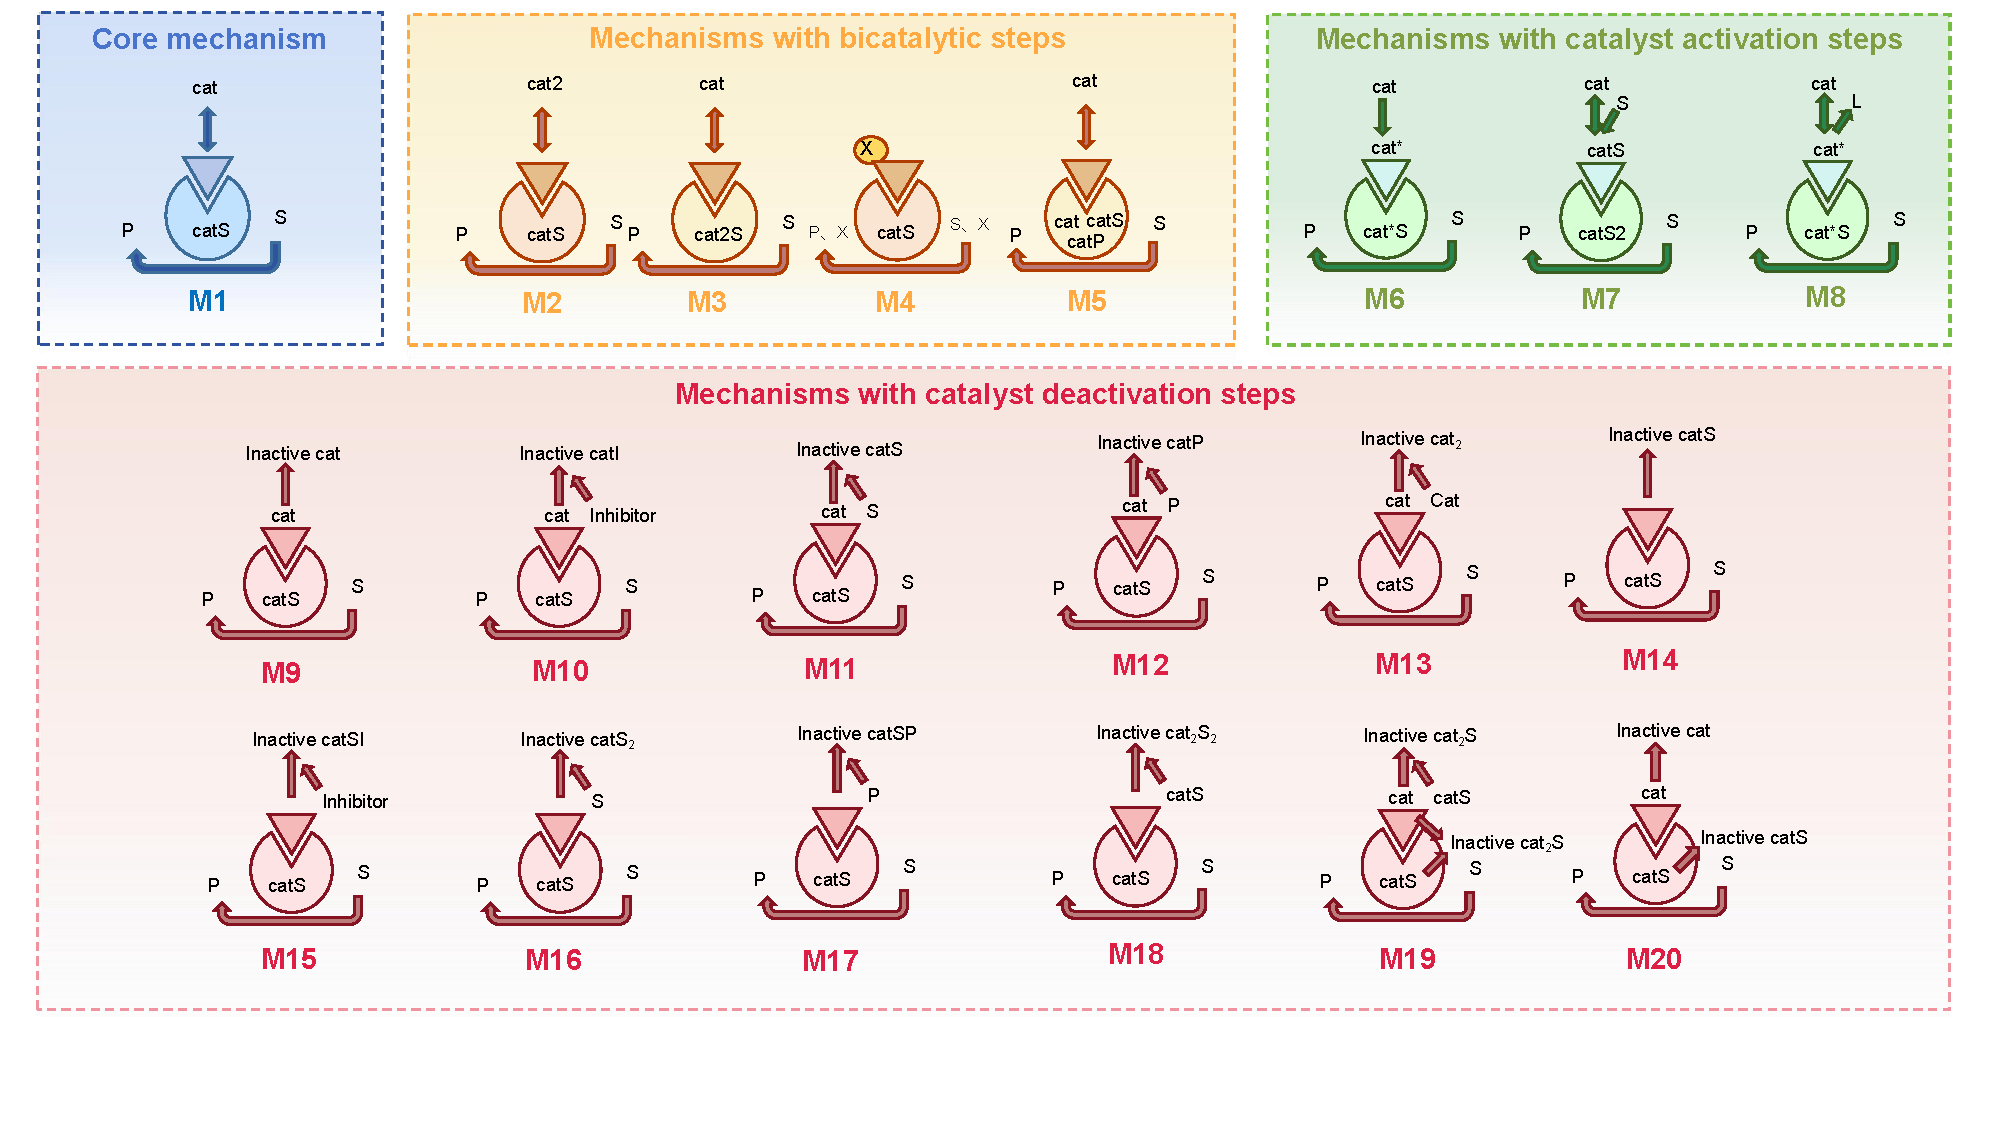
\includegraphics[width=\textwidth]{data_generation/catalytic_mechanisms_types_M1_to_M20.pdf}
    \caption{Overview of the twenty catalytic mechanisms}
    \label{fig:catalytic_mechanisms_overview}
\end{figure}


\section{Parameter-space Sampling}
\label{sec:parameter_space_sampling}

Following the mathematical representation of each catalytic mechanism in section~\ref{sec:ODE_formalism}, kinetic parameter sets capable of generating kinetically distinct trajectories are identified by initially sampling a preliminary pool of $108{,}208 / 20 = 5{,}410$ candidate parameter vectors for each mechanism. The rate constant $k_i$ within these vectors are independently drawn from a log-uniform distribution defined by:

\begin{equation}
k_i \sim 10^{\mathcal{U}(\log_{10}10^{-5}, \log_{10}10^{5})},
\end{equation}
and subsequently rounded to three significant figures to eliminate numerical precision beyond physical and computational significance ~\cite{Novak2018}. This broad parameter range encompasses kinetic regimes from slow to rapid reactions, thereby ensuring diverse mechanistic behaviors within the dataset.\\

Candidate parameter vectors are then evaluated through a multi-stage filtering procedure. Firstly, parameter sets must satisfy a maximum-yield criterion, requiring the substrate batch conversion at the reaction endpoint to fall within the range:

\begin{equation}
X_S = \frac{[S]_0 - [S]_{t_{\text{max}}}}{[S]_0}, \quad \text{subject to} \quad 0.5 \leq X_S \leq 1.0,
\end{equation}
where $[S]_0$ is the initial substrate concentration at $t = 0$, and $[S]_{t_{\text{max}}}$ is the remaining substrate concentration at the end of the reaction time ($t_{\text{max}} = 100$). This criterion facilitates the generation of trajectories that capture meaningful kinetic transients rather than trivial conversions lacking mechanistic information. Additionally, each parameter vector is subjected to mechanism-specific filtering conditions detailed in section~\ref{sec:mechanism_specific_parameter_selection_criteria}, guaranteeing that the retained parameter sets exhibit uniquely identifiable mechanistic signatures. Finally, any parameter vectors appearing simultaneously in multiple catalytic mechanisms are discarded, thereby maintaining mutual exclusivity among mechanism labels within the dataset.\\

In cases where direct log-uniform sampling proves inefficient—yielding prohibitively low acceptance rates—a biased sampling strategy is employed. For example, in mechanism \textbf{M2}, where kinetics depend on the balance between dimer association and dissociation, most parameter sets fail to achieve sufficient catalyst dimer (\emph{cat\textsubscript{2}}) accumulation. Physically, the association rates ($k_2$) must be sufficiently fast to generate a detectable dimer population, whereas the dissociation rates ($k_{-2}$) and turnover steps ($k_3$, $k_{-3}$) must remain balanced to avoid complete sequestration of active catalyst. Studies of organocatalytic systems demonstrate that inactive dimeric aggregates dominate under conditions where this balance is lost, severely limiting catalytic efficiency ~\cite{Ali2022, Ford2016}. This constraint drastically reduces the proportion of valid parameter set, a challenge previously highlighted by recent microkinetic sensitivity analyses ~\cite{Motagamwala2021}. Recent advances in rare-event sampling have demonstrated that tailored biasing strategies significantly enhance acceptance rates in rugged kinetic landscapes. For instance, Bolhuis developed an adaptive sampler that concentrates proposals in regions of parameter space likely to support productive aggregate formation, accelerating convergence by several orders of magnitude ~\cite{Bolhuis2025}.\\

However, due to the absence of detailed chemical domain expertise and relevant industry experience, this study was unable to leverage mechanistic priors and externally calibrated rate estimates to guide the parameter-space sampling. Consequently, an iterative narrowing strategy was adopted, progressively refining each kinetic parameter range until both the accumulation of the catalyst dimer (\emph{cat\textsubscript{2}}) and the overall substrate conversion consistently satisfied the acceptance criteria. Specifically, given the computational constraints defined by the maximum of 500 sampling rounds, each evaluating up to 200 candidate parameter sets (resulting in a total maximum of 100,000 parameter evaluations), an acceptance rate exceeding approximately 5.41\% was necessary to ensure the collection of at least 5,410 valid parameter combinations per mechanism. After four iterative rounds of parameter-range refinement, the acceptance rate for mechanism \textbf{M2} improved significantly, reaching approximately 12.6\%. The final biased parameter sampling ranges for mechanism \textbf{M2} are explicitly given by:

\begin{equation}
\boldsymbol{\theta}^{\mathrm{M2}} 
= (k_1, k_{-1}, k_2, k_{-2}, k_3, k_{-3})^{\top}, \quad
\text{with} \quad
\begin{array}{ll}
k_1,\; k_{-1} &\sim \mathcal{U}(0.9, 1.8), \\
k_2 &\sim \mathcal{U}(3.2, 5.0), \\
k_{-2} &\sim \mathcal{U}(0.018, 0.043), \\
k_3 &\sim \mathcal{U}(0.022, 0.13), \\
k_{-3} &\sim \mathcal{U}(0.17, 1.5).
\end{array}
\label{eq:M2_biased_sampler}
\end{equation}

Although this iterative refinement strategy appear relatively crude compared to methods informed by mechanistic insight or empirical industrial benchmarks, it substantially improves the sampling efficiency while preserving the diversity of mechanistically valid kinetic profiles. Similar biased sampling procedures were applied to other catalytic reaction mechanisms exhibiting comparable sampling challenges, with each mechanism requiring tailored iterative narrowing based on its specific mechanistic constraints.



\section{Mechanism-Specific Parameter Selection Criteria}
\label{sec:mechanism_specific_parameter_selection_criteria}

As described in section~\ref{sec:parameter_space_sampling}, after satisfying the initial maximum-yield criterion, each candidate parameter vector undergoes further evaluation based on additional mechanism-specific filtering conditions. These criteria are individually tailored to the unique kinetic characteristics and constraints of mechanisms \textbf{M1–M20}. Ultimately, parameter vectors are included in the final dataset only if their simulated kinetic trajectories fully meet these rigorous mechanism-specific post-filtering requirements.\\

For the core mechanism (\textbf{M1}), all kinetic parameter sets are admissible without additional mechanistic restrictions. In contrast, for mechanisms with bicatalytic steps, such as \textbf{M2}, parameters are retained only if the fraction of the dimeric catalyst species (\emph{cat\textsubscript{2}}) exceeds 10\% of the total catalyst concentration within the substrate conversion interval. An illustrative example Figure~\ref{fig:M2_criterion} is provided below.

\begin{figure}[H]
    \hspace*{-5pt}
    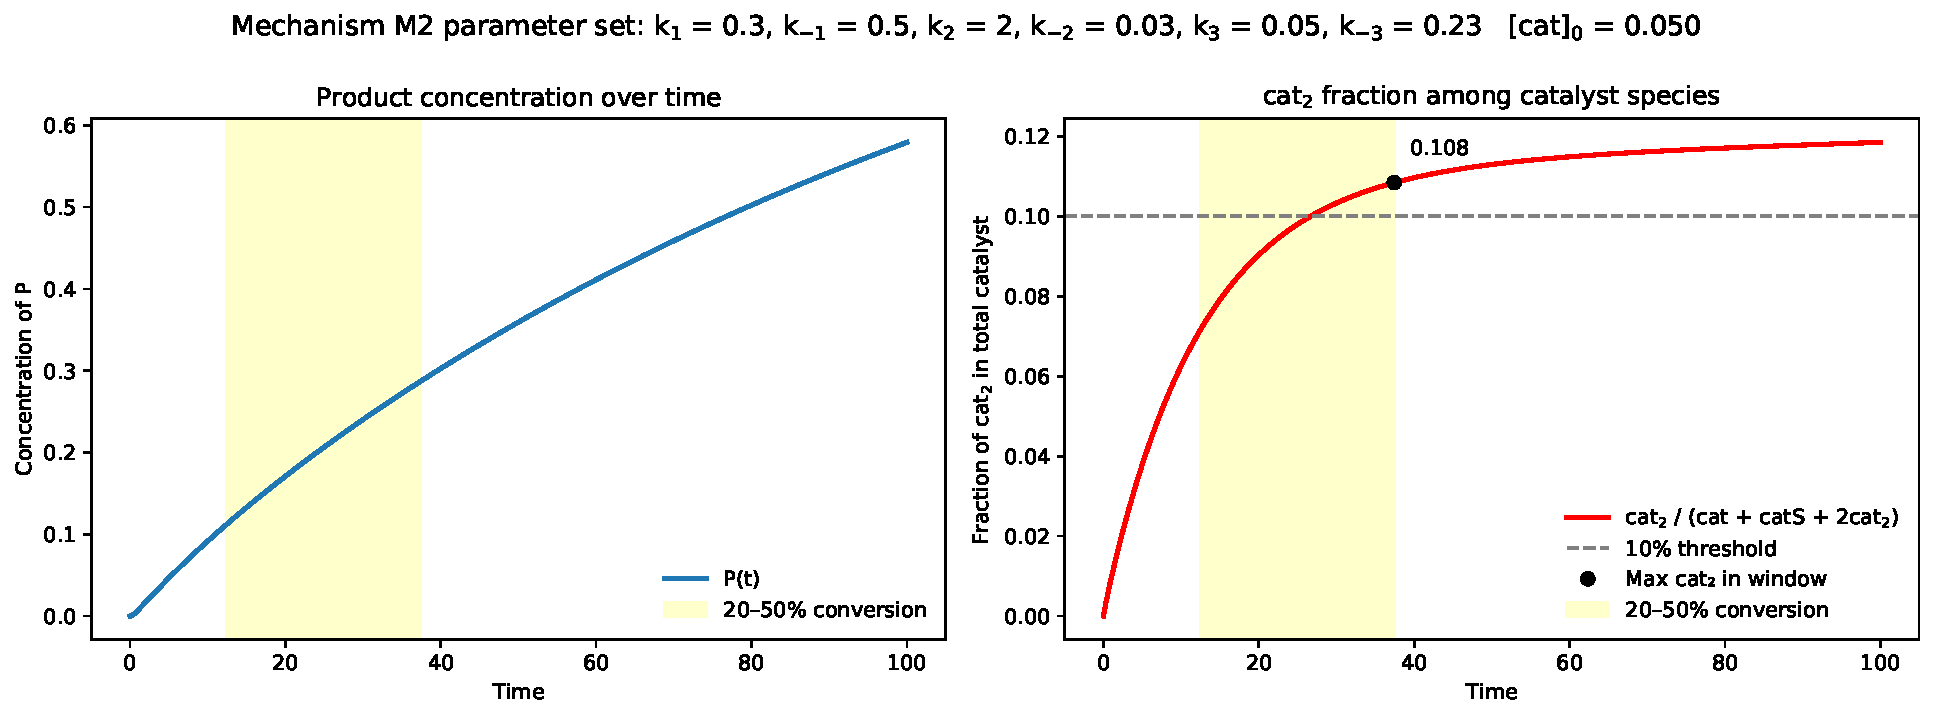
\includegraphics[width=0.95\textwidth]{data_generation/M2.pdf}
    \caption{Example of filtering criterion for mechanism M2}
    \label{fig:M2_criterion}
\end{figure}

The left panel shows the evolution of product concentration $P(t)$ over time. The right panel depicts the fraction of \emph{cat\textsubscript{2}} relative to the total catalyst concentration (\emph{cat} + \emph{catS} + 2·\emph{cat\textsubscript{2}}). The maximum fraction (10.8\%, black dot) within the 20–50\% conversion window exceeds the 10\% threshold (dashed line), and thus this parameter set is accepted into the dataset.\\

This filtering retains parameter sets with significant accumulation of dimeric catalyst species (\emph{cat\textsubscript{2}}), which are labeled as \textbf{M2}. Dimer formation is known to introduce nonlinear catalyst dependence and alter the reaction order, generating a kinetic “fingerprint” distinct from the monomeric mechanism (\textbf{M1}) ~\cite{Rosner2001}. However, if the fraction of \emph{cat\textsubscript{2}} remains low, the bicatalytic pathway serves as a minor off-cycle reservoir with negligible effect on the overall catalytic flux ~\cite{Rai2024}. In such cases, the $P(t)$ profiles align with \textbf{M1} after rate constant adjustment, rendering \textbf{M2} indistinguishable within experimental noise ~\cite{Sahharova2023}.  
Similarly, mechanisms with catalyst activation steps require criteria to ensure moderate accumulation of active species. For instance, in mechanism \textbf{M6}, parameter sets are retained only when the fraction of activated species (\emph{cat*} + \emph{cat*S}) constitutes 10–90\% of the total catalyst at 20\% conversion (Figure~\ref{fig:M6_criterion}).




\begin{figure}[H]
    \centering
    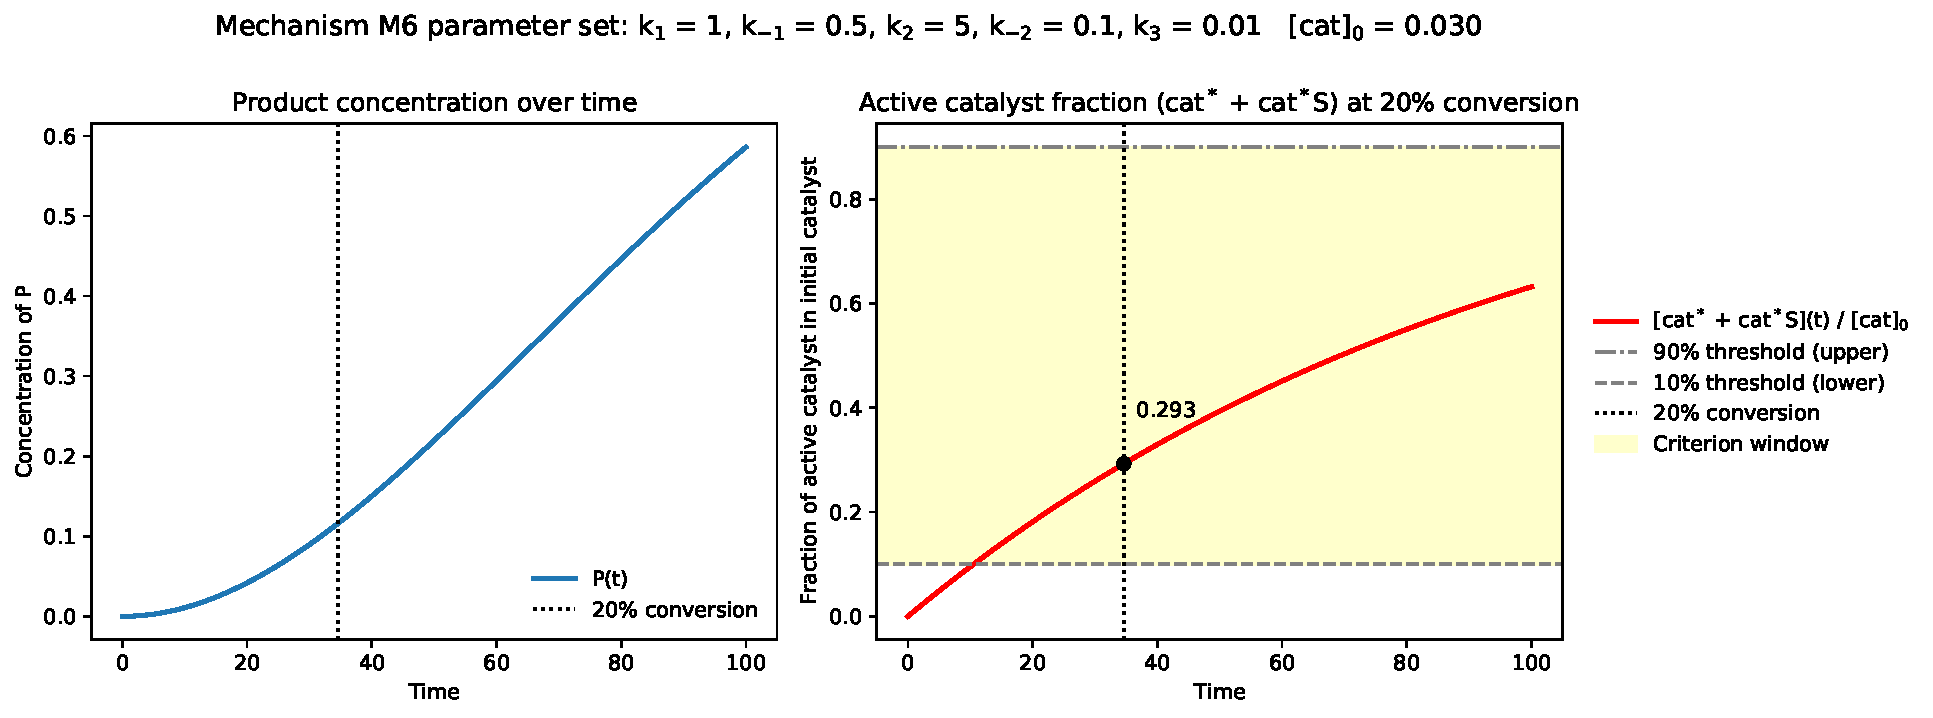
\includegraphics[width=\textwidth]{data_generation/M6.pdf}
    \caption{Example of filtering criterion for mechanism M6}
    \label{fig:M6_criterion}
\end{figure}

This criterion window excludes scenarios with either instantaneous activation—rendering M6 indistinguishable from the core mechanism—or sluggish activation with minimal formation of active species. Restricting the active-catalyst fraction to 10–90 \% at 20\% conversion defines a regime with an observable induction period and stable steady-state population of active species. Such conditions have been identified by microkinetic modeling and continuous-addition kinetic elucidation (CAKE) experiments as prerequisites for extracting meaningful catalyst orders and speciation parameters ~\cite{Williams2023}. Similarly, mechanisms with catalyst deactivation steps require criteria to ensure moderate accumulation of active species. For example, in mechanism \textbf{M9}, a parameter set is accepted only if active species (\emph{cat} + \emph{catS}) remains between 50\% and 90\% of the initial catalyst at 50\% conversion, as shown in Figure~\ref{fig:M9_criterion}.


\begin{figure}[H]
    \centering
    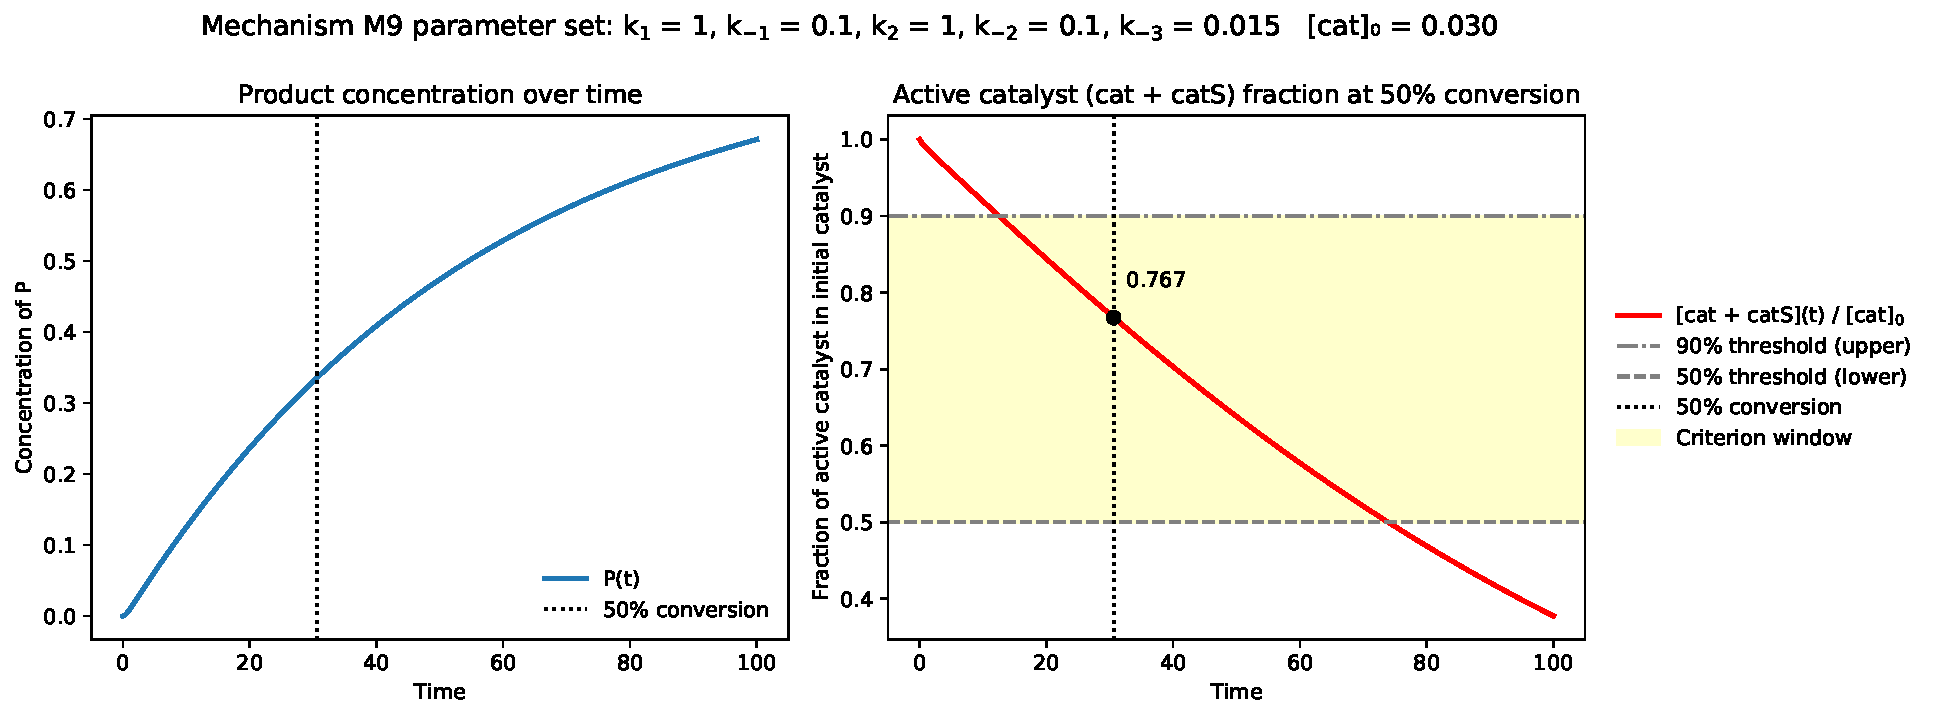
\includegraphics[width=\textwidth]{data_generation/M9.pdf}
    \caption{Example of filtering criterion for mechanism M9}
    \label{fig:M9_criterion}
\end{figure}


According to Martínez-Carrión et al.\ (2019), rigorous kinetic methodologies such as variable-time normalization analysis (VTNA) reliably distinguish catalyst deactivation pathways only if the experimental kinetic data exhibit an intermediate, measurable decline in catalyst activity~\cite{MartinezCarrion2019}. Specifically, minimal ($<$10\%) or excessive ($>$50\%) losses in catalyst activity obscure the distinct kinetic signatures required for reliable parameter estimation. Thus, the \textbf{M9} filtering criterion was explicitly designed based on these considerations, selecting parameter sets that align precisely within this intermediate activity-loss window.

\section{Numerical Integration and Solver Configuration}
\label{sec:numerical_integration}

Having defined the ODE representations in section~\ref{sec:ODE_formalism} and established a rigorous kinetic parameter sampling and filtering procedure (section~\ref{sec:parameter_space_sampling}–~\ref{sec:mechanism_specific_parameter_selection_criteria}), the next is the numerical integration of these ODE systems to generate concentration–time trajectories. Numerical integration for all catalytic mechanisms was performed using SciPy’s \texttt{solve\_ivp} function with the LSODA integration method. LSODA is an adaptive integrator capable of automatically detecting stiffness and dynamically switching between Adams methods (appropriate for non-stiff equations) and Backward Differentiation Formulas (BDF, suitable for stiff equations). For each valid parameter vector, the solver configuration is defined as follows:

\begin{equation}
\texttt{solve\_ivp}\left(\frac{d\mathbf{C}(t)}{dt} = \mathbf{f}(\mathbf{C}(t), \boldsymbol{\theta});\ 
t \in [0, t_{\max}];\ 
\mathbf{C}(0) = \mathbf{C}_0;\ \texttt{rtol}=10^{-6};\ \texttt{atol}=10^{-9} \right).
\end{equation}

Solver accuracy was controlled by setting a relative tolerance (\texttt{rtol}) of $10^{-6}$ and an absolute tolerance (\texttt{atol}) of $10^{-9}$. These tight tolerances were selected to minimize numerical errors and ensure strict mass and energy conservation across the wide kinetic parameter range investigated ($10^{-5}$ to $10^{5}$). Specifically, Goodwin et al. (2017) demonstrated that rigorous control of numerical tolerances is essential in chemical kinetic modeling to avoid artificial mass imbalances and energy drift, directly validating our choice of strict error settings~\cite{Goodwin2017}. Additionally, the solver’s maximum step size was explicitly restricted to 1.0 s, effectively mitigating numerical overshoot during rapid substrate conversions and abrupt catalyst activation or deactivation events. Stewart and Bair (2013) explicitly support the use of such step-size constraints to maintain numerical stability in highly reactive chemical systems~\cite{Stewart2013}.\\

Parameter sets yielding solver failures, non-finite values, or NaNs  were discarded to maintain numerical stability and physical plausibility. This filtering criterion aligns with Rackauckas and Nie (2017), who advocate stringent rejection of non-physical or unstable numerical solutions in extensive parameter space explorations~\cite{Rackauckas2017}. The solver outputs were sampled at 5,000 uniform time points, providing adequate temporal resolution to capture rapid transient dynamics without excessive computational cost, as explicitly recommended by Pontrelli et al. (2022) in their guidelines for stiff biochemical kinetic models~\cite{Pontrelli2022}.

\section{Initial Condition Design}
\label{sec:initial_condition_design}

The trajectories obtained in Section~\ref{sec:numerical_integration} are converted into fixed-size tensors appropriate for subsequent deep learning tasks by pairing each kinetic parameter vector with an ensemble of initial conditions. For every mechanism, a pool of thirty catalyst loadings is first generated by drawing:

\begin{equation}
\operatorname{cat}_0^{\text{tarin/val}} \;\sim\; \mathcal{U}(0.01,\,0.10)\quad\text{(mol fraction)}
\end{equation}
and sorting them in ascending order, thereby guaranteeing monotonicity that later facilitates indexing operations~\cite{Brown2017}.  Throughout the training and validation partitions the substrate and product are kept at their standard values,
\(
[S]_0 = 1.0,\ [P]_0 = 0,
\)
so that only the catalyst loading varies within the pool; such controlled variation in a single kinetic factor has been shown to sharpen the sensitivity of deep learning models to catalyst‐dependent rate laws~\cite{Esterby2020,Olsson2019}.\\

For each kinetic parameter set, four distinct reaction trajectories are generated. The first three trajectories correspond to three distinct catalyst loadings—low, medium, and high—sampled from a predefined pool of thirty possible initial catalyst concentrations, while maintaining the standard initial conditions $(S_0,P_0)$. Subsequently, a fourth ``perturbed" trajectory is  generated by selecting one of these three catalyst loadings and initializing the reaction from a partially converted state. Specifically, the initial substrate concentration for this trajectory is randomly sampled as:


\begin{equation}
S_0^{(4)}\sim \mathcal{U}(0.4,\,0.8)
\end{equation}
with the product concentration set to its stoichiometric complement
\(
P_0^{(4)} = 1 - S_0^{(4)}.
\)
The inclusion of this partially converted initial state introduces realistic variability resembling mid-batch sampling and has been demonstrated to improve the generalisation of kinetic models to unseen conversion regimes~\cite{Rothenberg2024,Guo2024}.\\ 

The test partition preserves the same four-trajectory structure but employs a distinct sampling strategy specifically designed to assess the extrapolation capability of the trained models. In this partition, three ``standard" trajectories again use the fixed initial substrate and product conditions ($[S]_0=1.0,\ [P]_0=0$), yet their catalyst loadings are sampled from three narrow intervals, chosen to represent catalyst concentrations that were infrequently encountered during model training:

\begin{equation}
\operatorname{cat}_0^{\text{test}} \sim
\begin{cases}
\mathcal{U}(0.01, 0.02), & \text{(low catalyst regime)} \\[4pt]
\mathcal{U}(0.045, 0.055), & \text{(intermediate catalyst regime)} \\[4pt]
\mathcal{U}(0.09, 0.10). & \text{(high catalyst regime)}
\end{cases}
\end{equation}

The deliberate choice of catalyst loadings from these three narrowly bounded regimes forces the evaluation set to deviate from the densely sampled training region, introducing a controlled covariate condition shift. This design enables the test partition to interrogate whether the learned kinetic representations remain valid  under extrapolation to rarely or unseen catalyst regimes. Recent work has demonstrated that even state-of-the-art machine learning models—particularly in chemical kinetics and reaction modeling—tend to memorize rather than generalize kinetic patterns, failing to extrapolate beyond the training manifold.~\cite{Guo2024}. By evaluating under these rare catalyst loadings, the test partition offers a rigorous diagnostic of the model’s ability to infer underlying reaction rules rather than overfitting to training distributions.\\ 

\section{Time-Resolved Tensor Construction}
\label{sec:time_resolved_tensor_construction}

The preceding section (Section~\ref{sec:initial_condition_design}) established a four‑trajectory ensemble for every valid kinetic parameter set, thereby embedding controlled variation in catalyst loading and conversion states into the dataset. Building upon this ensemble, the current subsection details the process by which each high-resolution trajectory is compressed into a fixed-size tensor suitable for input into deep neural networks.\\

All generated trajectories are first numerically integrated over a dense temporal comprising $5{,}000$ uniformly spaced points spanning the complete integration interval ($t \in [0, t_{\max}]$). Subsequently, these high-resolution trajectories undergo uniform temporal subsampling, reducing the number of retained data points to a computationally efficient cardinality:

\begin{equation}
N_t=
\begin{cases}
21 & \text{(training / validation)},\\[4pt]
7  & \text{(test)},
\end{cases}
\end{equation}
where the initial time point $t=0$ is always retained, while the remaining $N_t-1$ points are sampled without replacement from the interior of the integration interval. This approach ensures accurate capture of rapid transient behaviors at early times, which frequently contain critical rate-determining information \cite{Goodwin2017}.\\

The more aggressive subsampling applied to the test partition (seven data point) deliberately mimics the sparse and noisy time series data typically encountered in in-situ spectroscopic monitoring, where measurement frequency is restricted by instrument duty cycles~\cite{Lim2021}. Evaluating model performance under these challenging conditions assesses robustness against covariate shift and observation sparsity, effectively testing generalization beyond the dense, low-noise conditions encountered during training~\cite{Appleby2024}.\\

Each subsampled trajectory consists of columns representing time, substrate concentration, and product concentration. These three columns are then stacked across the four trajectories associated with the same kinetic parameter vector, resulting in:

\begin{equation}
\mathbf{X}_{2} \;=\;
\bigl[
\{t,S,P\}^{\!\top}_{1}\!,
\;
\{t,S,P\}^{\!\top}_{2}\!,
\;
\{t,S,P\}^{\!\top}_{3}\!,
\;
\{t,S,P\}^{\!\top}_{4}
\bigr]
\;\in\;
\mathbb{R}^{\,N_t\times 12}.
\end{equation}
Each time column has been rescaled to the unit interval using a simple min–max transformation:
\begin{equation}
t^{\mathrm{norm}} = \frac{t - \min(t)}{\max(t)-\min(t)},
\end{equation}
thereby removing the absolute scale of the integration window from the learning task. Min–max scaling accelerates gradient-based optimization, mitigates internal covariate shift, and reduces the propagation of experimental noise; recent kinetic surrogate benchmarks have demonstrated that this scaling reduces convergence times by nearly 50\% compared to unscaled inputs, while simultaneously enhancing predictive robustness \cite{Dong2025}. Conversely, substrate and product concentrations remain in their physical units, enabling the neural network to learn chemically meaningful absolute scales.

\section{Final Dataset Integration}
\label{sec:final_dataset_integration}

In previous sections, mechanistically valid kinetic trajectories were constructed and compressed into fixed-size, time-resolved tensors. The concluding step in the simulation data generation workflow concatenates these mechanism-specific samples into training, validation, and test sets, while normalising metadata and exporting the results in a format suitable for training downstream classification models.\\

All samples derived from the twenty mechanisms are first padded so that every kinetic parameter vector \( \boldsymbol{\theta} \) attains the uniform maximum length:
\begin{equation}
d_{\max} = \max_{i \in [1,20]} d_i = 6,
\end{equation}
where \( d_i \) denotes the intrinsic dimensionality of mechanism \( M_i \). Padding with \texttt{NaN} preserves parameter dimensionality without introducing numerical bias. The catalyst-loading vector \( \mathbf{x}_1 \in \mathbb{R}^{4} \) remains unchanged, while the concentration tensor \( \mathbf{X}_2 \in \mathbb{R}^{N_t \times 12} \) undergoes min–max scaling in its time columns, retaining substrate and product concentrations in their physical units. Mechanism labels are encoded as one-hot vectors \( \mathbf{y} \in \{0,1\}^{20} \), framing the downstream neural-network task as a twenty-class classification.\\

After aggregation, the corpus sizes satisfy  \( N_{\text{train}} = 4{,}950{,}000 \), \( N_{\text{val}} = 50{,}000 \), and \( N_{\text{test}} = 100{,}000 \) samples, with corresponding tensor dimensions given by:

\[
\begin{aligned}
&\mathbf{x}_1^{\text{train}} \in \mathbb{R}^{\,4\,950\,000\times 4}, &
&\mathbf{X}_2^{\text{train}} \in \mathbb{R}^{\,4\,950\,000\times 21\times 12}, &
&\mathbf{y}^{\text{train}} \in \mathbb{R}^{\,4\,950\,000\times 20}, \\[0.5em]
&\mathbf{x}_1^{\text{val}} \in \mathbb{R}^{\,50\,000\times 4}, &
&\mathbf{X}_2^{\text{val}} \in \mathbb{R}^{\,50\,000\times 21\times 12}, &
&\mathbf{y}^{\text{val}} \in \mathbb{R}^{\,50\,000\times 20}, \\[0.5em]
&\mathbf{x}_1^{\text{test}} \in \mathbb{R}^{\,100\,000\times 4}, &
&\mathbf{X}_2^{\text{test}} \in \mathbb{R}^{\,100\,000\times 7\times 12}, &
&\mathbf{y}^{\text{test}} \in \mathbb{R}^{\,100\,000\times 20}.
\end{aligned}
\]

\vspace{0.2cm}
Figure~\ref{fig:kinetic_profile_sample} presents a randomly selected entry from the training corpus. Four kinetic profiles are displayed—three initiated from the standard substrate concentration with distinct catalyst loadings, and one from a partially converted state—all originating from mechanism \textbf{M9}. The example demonstrates the diversity of kinetic behaviour captured by the dataset through constructed initial-state variations.

\begin{figure}[H]
    \centering
    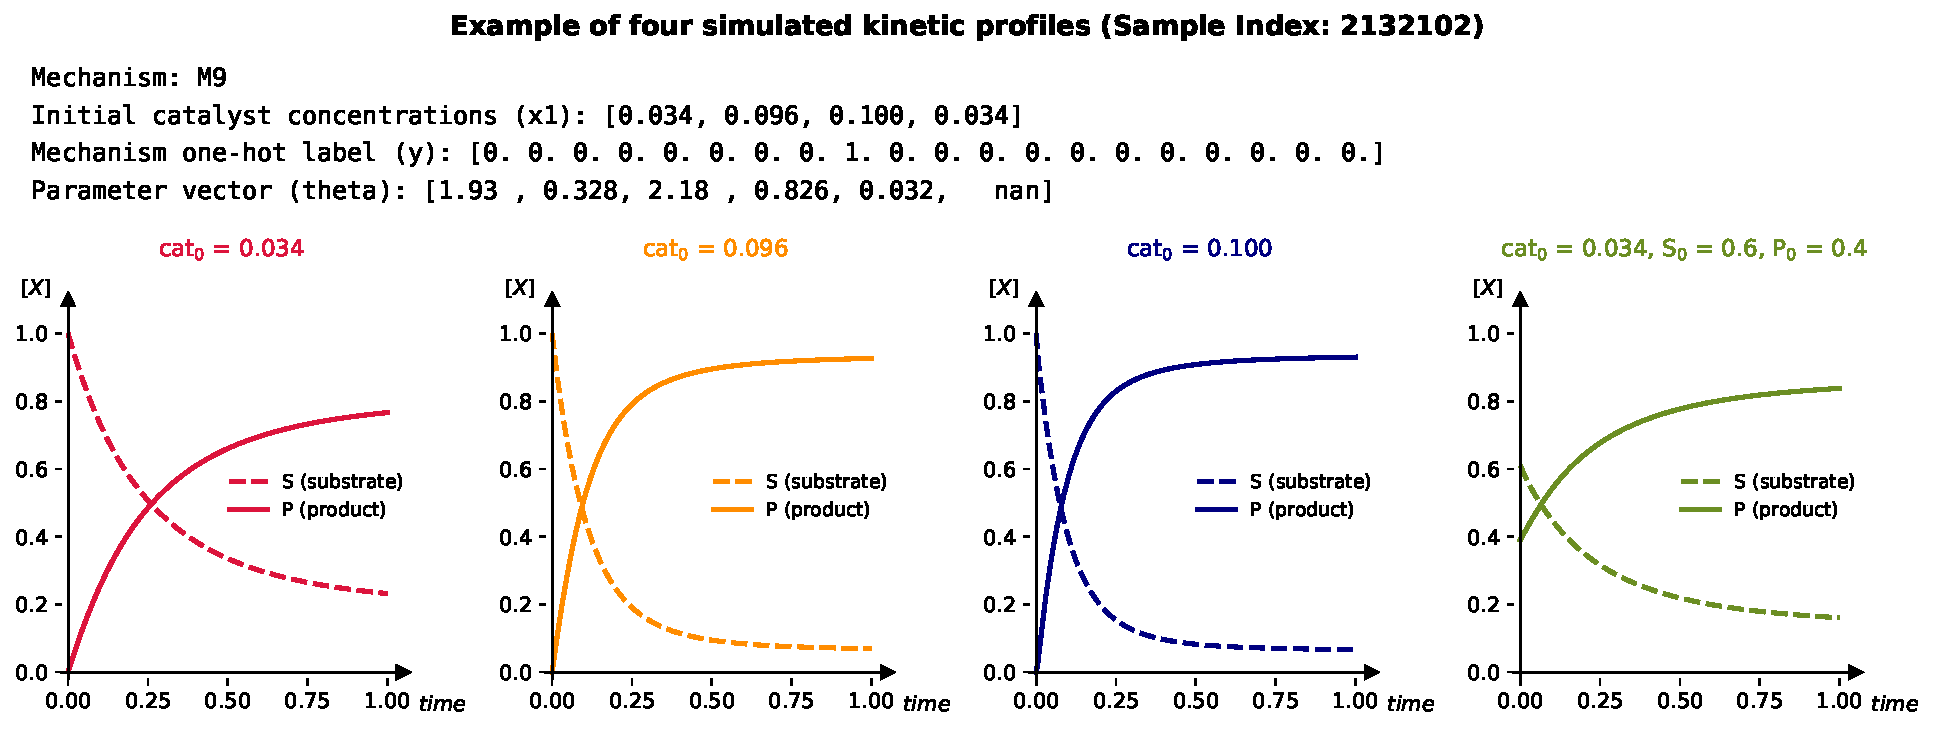
\includegraphics[width=\textwidth]{data_generation/kinetic_profile_sample.pdf}
    \caption{Kinetic trajectories for mechanism M9 under different initial conditions.}
    \label{fig:kinetic_profile_sample}
\end{figure}


% -----------------------------------------------------------------------------

\chapter{Critical Evaluation}
\label{chap:evaluation}

{\bf A topic-specific chapter, roughly 30\% of the total page-count} 
\vspace{1cm} 

\noindent
This chapter is intended to evaluate what you did.  The content is highly 
topic-specific, but for many projects will have flavours of the following:

\begin{enumerate}
\item functional  testing, including analysis and explanation of failure 
      cases,
\item behavioural testing, often including analysis of any results that 
      draw some form of conclusion wrt. the aims and objectives,
      and
\item evaluation of options and decisions within the project, and/or a
      comparison with alternatives.
\end{enumerate}

\noindent
This chapter often acts to differentiate project quality: even if the work
completed is of a high technical quality, critical yet objective evaluation 
and comparison of the outcomes is crucial.  In essence, the reader wants to
learn something, so the worst examples amount to simple statements of fact 
(e.g., ``graph X shows the result is Y''); the best examples are analytical 
and exploratory (e.g., ``graph X shows the result is Y, which means Z; this 
contradicts [1], which may be because I use a different assumption'').  As 
such, both positive {\em and}\/ negative outcomes are valid {\em if} presented 
in a suitable manner.

% -----------------------------------------------------------------------------

\chapter{Conclusion}
\label{chap:conclusion}

{\bf A compulsory chapter,  roughly 10\% of the total page-count}
\vspace{1cm} 

\noindent
The concluding chapter(s) of a dissertation are often underutilized because they're 
too often left too close to the deadline: it is important to allocate enough time and 
attention to closing off the story, the narrative, of your thesis.

Again, there is no single correct way of closing a thesis. 

One good way of doing this is to have a single chapter consisting of three parts:

\begin{enumerate}
\item (Re)summarise the main contributions and achievements, in essence
      summing up the content.
\item Clearly state the current project status (e.g., ``X is working, Y 
      is not'') and evaluate what has been achieved with respect to the 
      initial aims and objectives (e.g., ``I completed aim X outlined 
      previously, the evidence for this is within Chapter Y'').  There 
      is no problem including aims which were not completed, but it is 
      important to evaluate and/or justify why this is the case.
\item Outline any open problems or future plans.  Rather than treat this
      only as an exercise in what you {\em could} have done given more 
      time, try to focus on any unexplored options or interesting outcomes
      (e.g., ``my experiment for X gave counter-intuitive results, this 
      could be because Y and would form an interesting area for further 
      study'' or ``users found feature Z of my software difficult to use,
      which is obvious in hindsight but not during at design stage; to 
      resolve this, I could clearly apply the technique of Bloggs {\em et al.}.
\end{enumerate}

Alternatively, you might want to divide this content into two chapters: a penultimate chapter with a title such as ``Further Work" and then a final chapter ``Conclusions". Again, there is no hard and fast rule, we trust you to make the right decision. 

And this, the final paragraph of this thesis template, is just a bunch of citations, added to show how to generate a BibTeX bibliography. Sources that have been randomly chosen to be cited here include:
~\cite{miller_etal_2018_clojure,webber_marwan_2015,touretzky_2013_lisp,eckmann_etal_1987,marwan_2011,vach_2015,shiller_2017,vytelingum_2006,tesfatsion_2002,rust_etal_1992}.




% =============================================================================

% Finally, after the main matter, the back matter is specified.  This is
% typically populated with just the bibliography.  LaTeX deals with these
% in one of two ways, namely
%
% - inline, which roughly means the author specifies entries using the 
%   \bibitem macro and typesets them manually, or
% - using BiBTeX, which means entries are contained in a separate file
%   (which is essentially a database) then imported; this is the 
%   approach used below, with the databased being dissertation.bib.
%
% Either way, the each entry has a key (or identifier) which can be used
% in the main matter to cite it, e.g., ~\cite{X}, ~\cite[Chapter 2}{Y}.

\backmatter

\bibliography{sample_bibtex.bib}

% -----------------------------------------------------------------------------

% The dissertation concludes with a set of (optional) appendices; these are 
% the same as chapters in a sense, but once signalled as being appendices via
% the associated macro, LaTeX manages them appropriately.

\appendix

\chapter{An Example Appendix}
\label{appx:example}

Content which is not central to, but may enhance the dissertation can be 
included in one or more appendices; examples include, but are not limited
to

\begin{itemize}
\item lengthy mathematical proofs, numerical or graphical results which 
      are summarised in the main body,
\item sample or example calculations, 
      and
\item results of user studies or questionnaires.
\end{itemize}

\noindent
Note that in line with most research conferences, the examiners are not
obliged to read such appendices.

% =============================================================================

\end{document}
